% Compile from the REPORT REPOSITORY ROOT, not from slides/.
% All figure paths are local to this repository; no ML-repository dependencies.
\documentclass[aspectratio=169]{beamer}
\usepackage[T1]{fontenc}
\usepackage[utf8]{inputenc}
\usepackage{lmodern}
\usepackage{booktabs,array,tabularx}
\usepackage{amsmath,amssymb}
\usepackage{graphicx}
\usepackage{tikz}
\usetikzlibrary{arrows.meta,positioning}
\IfFileExists{beamerthememetropolis.sty}{%
  \usetheme[progressbar=none,numbering=none]{metropolis}
}{\usetheme{default}}
\usefonttheme{professionalfonts}
\renewcommand{\sfdefault}{lmss}
\definecolor{Navy}{HTML}{142B45}
\definecolor{Blue}{HTML}{2767A6}
\definecolor{Pale}{HTML}{EAF1F7}
\definecolor{Muted}{HTML}{526679}
\setbeamercolor{normal text}{fg=Navy,bg=white}
\setbeamercolor{structure}{fg=Blue}
\setbeamercolor{frametitle}{fg=Navy,bg=white}
\setbeamercolor{alerted text}{fg=Blue}
\setbeamercolor{block title}{fg=Navy,bg=Pale}
\setbeamercolor{block body}{fg=Navy,bg=Pale}
\setbeamercolor{itemize item}{fg=Blue}
\setbeamerfont{normal text}{size=\fontsize{10.5}{13}}
\setbeamerfont{frametitle}{size=\fontsize{15.5}{19},series=\bfseries}
\setbeamersize{text margin left=7mm,text margin right=7mm}
\setbeamertemplate{navigation symbols}{}
\setbeamertemplate{itemize items}[circle]
\setbeamertemplate{frametitle}{%
  \vspace{1mm}\insertframetitle\par\vspace{.7mm}
  {\color{Blue}\rule{\textwidth}{0.6pt}}}
\newcommand{\footmarker}{\insertframenumber\,/\,18}
\setbeamertemplate{footline}{%
  \vbox to 17pt{%
    \vfill
    \hbox to\paperwidth{\hspace{7mm}{\color{Muted}\fontsize{7.5}{9}\selectfont
      NEU\enspace /\enspace MACHINE LEARNING\enspace /\enspace TETOUAN}%
      \hfill{\color{Muted}\fontsize{8}{9}\selectfont\footmarker}\hspace{7mm}}%
    \vskip3pt}}
\setlength{\tabcolsep}{5pt}
\renewcommand{\arraystretch}{1.2}
\newcommand{\takeaway}[1]{\par\vspace{1mm}{\color{Blue}\bfseries #1}\par}
\newcommand{\tagline}[1]{{\color{Blue}\fontsize{9}{11}\selectfont\bfseries #1}\par\vspace{1mm}}
\newcommand{\metric}[2]{{\color{Blue}\fontsize{25}{29}\selectfont\bfseries #1}\par{\small #2}\par}
\newcommand{\fig}[2]{\includegraphics[width=\linewidth,height=#2,keepaspectratio]{#1}}
% Generated from saved evidence; no model fitting.
\newcommand{\TestRMSE}{1,624.6}
\newcommand{\TestMAE}{1,094.6}
\newcommand{\TestMAPE}{1.78}
\newcommand{\TestRtwo}{0.9869}
\newcommand{\GainDaily}{50.7}
\newcommand{\GainWeekly}{38.0}
\newcommand{\CVRMSE}{2,410.6}
\newcommand{\CVSD}{766.3}
\newcommand{\HoneRMSE}{1,866.4}
\newcommand{\HoneGain}{22.6}
\newcommand{\DeltaTest}{1,419.1}
\newcommand{\Bias}{-202.1}
\newcommand{\WorstMAE}{4,579.2}
\newcommand{\TuningGain}{39.3}
\newcommand{\RFBefore}{9,168.1}
\newcommand{\RFAfter}{3,010.4}

\title{Machine Learning-Based Electricity Consumption Forecasting in Tetouan City}
\subtitle{A chronological evaluation of conventional regression models}
\author{Dang Nhat Minh \and Giang Hoang Son}
\institute{NATIONAL ECONOMICS UNIVERSITY}
\date{}
\hypersetup{pdftitle={Machine Learning-Based Electricity Consumption Forecasting in Tetouan City},
  pdfauthor={Dang Nhat Minh; Giang Hoang Son},pdfsubject={15-minute academic presentation},colorlinks=true,urlcolor=Blue}

\begin{document}
\usebeamerfont{normal text}

% MAIN 01 -- 25 seconds
\begin{frame}[plain]
\centering
\begin{minipage}{.91\textwidth}
\centering

\includegraphics[height=1.2cm,keepaspectratio]{report/assets/fda-logo.png}\hspace{3mm}%
\begin{minipage}{.77\textwidth}
\raggedright
{\fontsize{11}{13}\selectfont\bfseries NATIONAL ECONOMICS UNIVERSITY}\\
{\fontsize{10}{12}\selectfont Faculty of Data Science and Artificial Intelligence}\\
{\color{Blue}\small\bfseries MACHINE LEARNING}
\end{minipage}
\end{minipage}\\[5mm]
{\color{Navy}\fontsize{19}{23}\selectfont\bfseries
Machine Learning-Based Electricity\\[1mm]
Consumption Forecasting in Tetouan City}\\[1mm]
{\fontsize{11}{13}\selectfont A chronological evaluation of conventional regression models}\\[1mm]
{\color{Blue}\rule{.94\textwidth}{.7pt}}\\[1mm]
\begin{minipage}{.54\textwidth}
\raggedright\small
{\color{Blue}\bfseries GROUP MEMBERS}\\[1mm]
1. Dang Nhat Minh --- 11247196\\[-.5mm]
2. Giang Hoang Son --- 11247222
\end{minipage}\hfill
\begin{minipage}{.37\textwidth}
\raggedright\small
\textbf{Class:} DS66A\\[1mm]
\textbf{Instructor:} Ph.D. Luong Van Thien
\end{minipage}
\end{frame}

% MAIN 02 -- 35 seconds
\begin{frame}{Can machine learning beat a strong daily pattern?}
\tagline{PROBLEM MOTIVATION \& RESEARCH QUESTIONS}
Electricity planning needs the \textbf{shape of tomorrow's hourly demand}.
\vspace{2mm}
\begin{block}{The practical reference}
If demand repeats every day, copying yesterday is already competitive.
\end{block}
\vspace{2mm}
\begin{enumerate}
\setlength{\itemsep}{2mm}
\item How much do conventional models improve on seasonal baselines?
\item Which feature groups add predictive value?
\item How do tuning and the target formulation affect the result?
\end{enumerate}
\vspace{1mm}
{\small\color{Muted}Evaluate future periods and interpret gains against the named baseline.}
\end{frame}

% MAIN 03 -- 45 seconds
\begin{frame}{The target is mean hourly power across three zones}
\vspace{2mm}
\begin{columns}[c,onlytextwidth]
\column{.59\textwidth}
\[y_t=\frac{1}{6}\sum_{j=0}^{5}\bigl(Z_{1,t,j}+Z_{2,t,j}+Z_{3,t,j}\bigr)\quad[\mathrm{kW}]\]
\column{.37\textwidth}
{\small\textbf{52,416} ten-minute records\par
\textbf{8,736} hourly means\par
1 Jan--30 Dec 2017, Tetouan}
\end{columns}
\centering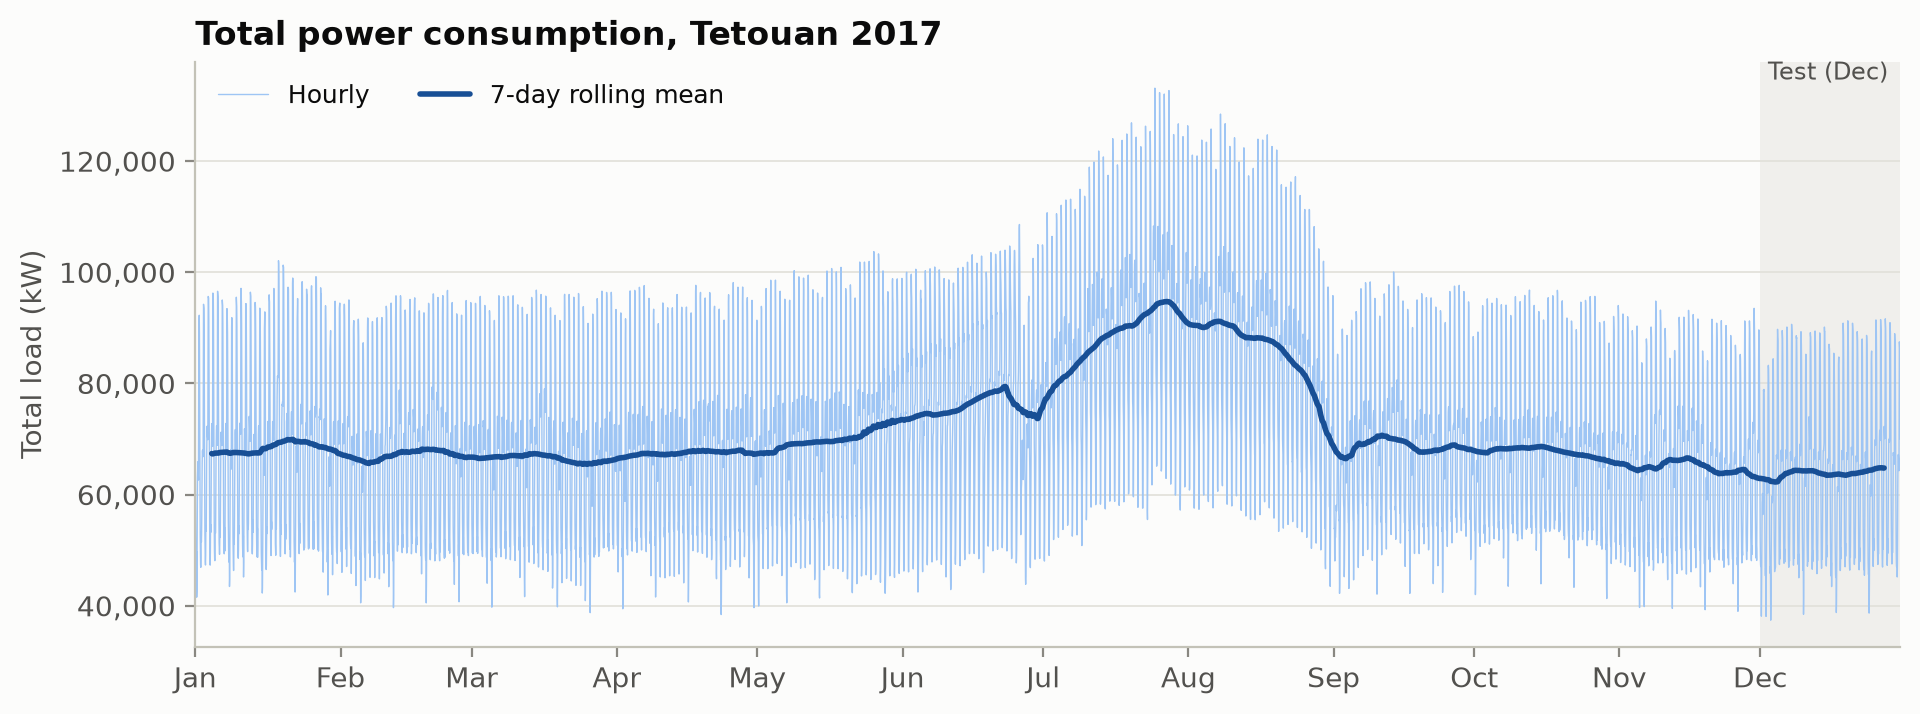
\includegraphics[width=\textwidth,height=3.55cm,keepaspectratio]{results/figures/F01_total_hourly_year.png}\par
\raggedright
{\small Mean power (kW); hourly energy is $y_t\times1\,\mathrm{h}$ (kWh).\par
Whole-year view includes December, but no 31 December data; the centred smooth is descriptive.}
\end{frame}

% MAIN 04 -- 35 seconds
\begin{frame}{Daily shape and season both matter}
\vspace{2mm}
\begin{columns}[c,onlytextwidth]
\column{.79\textwidth}
\fig{results/figures/F03_profile_by_season.png}{5.15cm}
\column{.18\textwidth}
\tagline{JANUARY--NOVEMBER}
\textbf{06--07h}\par daily minimum\par\vspace{4mm}
\textbf{19--20h}\par evening peak\par\vspace{4mm}
\textbf{Summer}\par higher load profile
\end{columns}
\par{\color{Blue}\bfseries Use calendar information and past load together.}\par
{\small\color{Muted}Profiles use January--November development data.}
\end{frame}

% MAIN 05 -- 50 seconds
\begin{frame}{Today looks like yesterday}
\setlength{\parskip}{2pt}
\tagline{JANUARY--NOVEMBER DATA ONLY}
\centering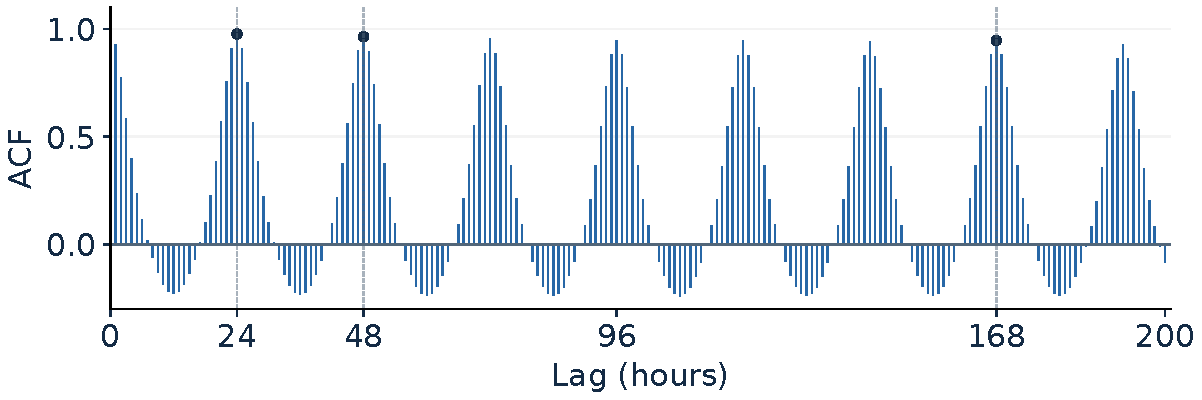
\includegraphics[width=\textwidth,height=3.15cm,keepaspectratio]{slides/figures/acf_view.pdf}\par
\raggedright
{\small ACF: \textbf{24 h = 0.98}, \textbf{48 h = 0.96}, \textbf{168 h = 0.95} (weekly peak).\par
Lag 12 h is negative: day and night are in opposite phases.\par
Copying yesterday (Naive-24h) is therefore a strong baseline.}
\takeaway{$\rightarrow$ features: \texttt{lag\_24}, \texttt{lag\_48} (daily history).}
\end{frame}

% MAIN 06 -- 55 seconds
\begin{frame}{Sundays and Mondays break the daily pattern}
\setlength{\parskip}{2pt}
\tagline{JANUARY--NOVEMBER / DIFFERENCE FROM MON--FRI AT THE SAME HOUR}
\begin{columns}[c,onlytextwidth]
\column{.52\textwidth}
\fig{slides/figures/weekday_difference.pdf}{5.0cm}
\column{.44\textwidth}
{\small Sundays: \textbf{5.9\% lower} on average; about \textbf{15\% lower at 7--8 h}.\par
Saturday mornings: \textbf{4--6\% lower}.\par
The effect varies by hour; a nonlinear model can learn this interaction.\par
Copying yesterday mismatches \textbf{Monday/Sunday} and \textbf{Sunday/Saturday}.}
\end{columns}
\takeaway{$\rightarrow$ features: \texttt{dayofweek}, \texttt{is\_weekend}, cyclic weekday.}
\end{frame}

% MAIN 07 -- 45 seconds
\begin{frame}{h24 and h1 use different information at issuance}
\begin{columns}[t,onlytextwidth]
\column{.48\textwidth}
\begin{block}{h24: midnight batch}
{\small 00:00 on day $D$: forecast its 24 hourly intervals.\par\vspace{1mm}
History: $y_{t-24},\ y_{t-48}$.\par\vspace{1mm}
\textbf{Lead to interval start: 0--23 h.}\par
Lead to interval completion: 1--24 h.}
\end{block}
\column{.48\textwidth}
\begin{block}{h1: hourly update}
{\small Update each hour for the next complete hourly interval.\par\vspace{1mm}
History: $y_{t-1},y_{t-2},y_{t-3},y_{t-24}$.\par\vspace{1mm}
Uses the latest completed-hour load.\par \textbf{Prompt measurements assumed}.}
\end{block}
\end{columns}
\vspace{1mm}
{\small The 24-hour lag is a minimum history offset; lead times vary across the daily batch.\par
Both settings assume prompt load measurements and use observed target-hour weather.}
\end{frame}

% MAIN 08 -- 40 seconds
\begin{frame}{Seventeen inputs combine timing, weather and history}
\tagline{MAIN h24 MODEL: FEATURE SET D}
{\renewcommand{\arraystretch}{1.07}
\begin{tabularx}{\textwidth}{@{}p{2.45cm}X>{\centering\arraybackslash}p{1.45cm}@{}}
\toprule
Group & Inputs & Count\\\midrule
Weather & Temperature, humidity, wind speed, general diffuse, diffuse & 5\\
Calendar & Hour, day of week, weekend; sine and cosine for hour and weekday & 7\\
Special days & Religious holiday, civil holiday, Ramadan indicators & 3\\
Daily history & $y_{t-24}$, $y_{t-48}$ & 2\\\bottomrule
\end{tabularx}
}\par\vspace{1mm}
{\color{Blue}\bfseries Target-hour observed weather requires forecasts at issuance.}\par\vspace{1mm}
{\small\color{Muted}History shifted; scalers fitted per fold. Weekly/rolling inputs excluded from set D.}
\end{frame}

% MAIN 09 -- 60 seconds
\begin{frame}{Model selection stays within January--November}
\vspace{1mm}
\begin{columns}[c,onlytextwidth]
\column{.63\textwidth}
\tagline{JAN--NOV DEVELOPMENT: 7,825 HOURS}
\column{.34\textwidth}
\tagline{DECEMBER TEST: 720 HOURS}
\end{columns}
\centering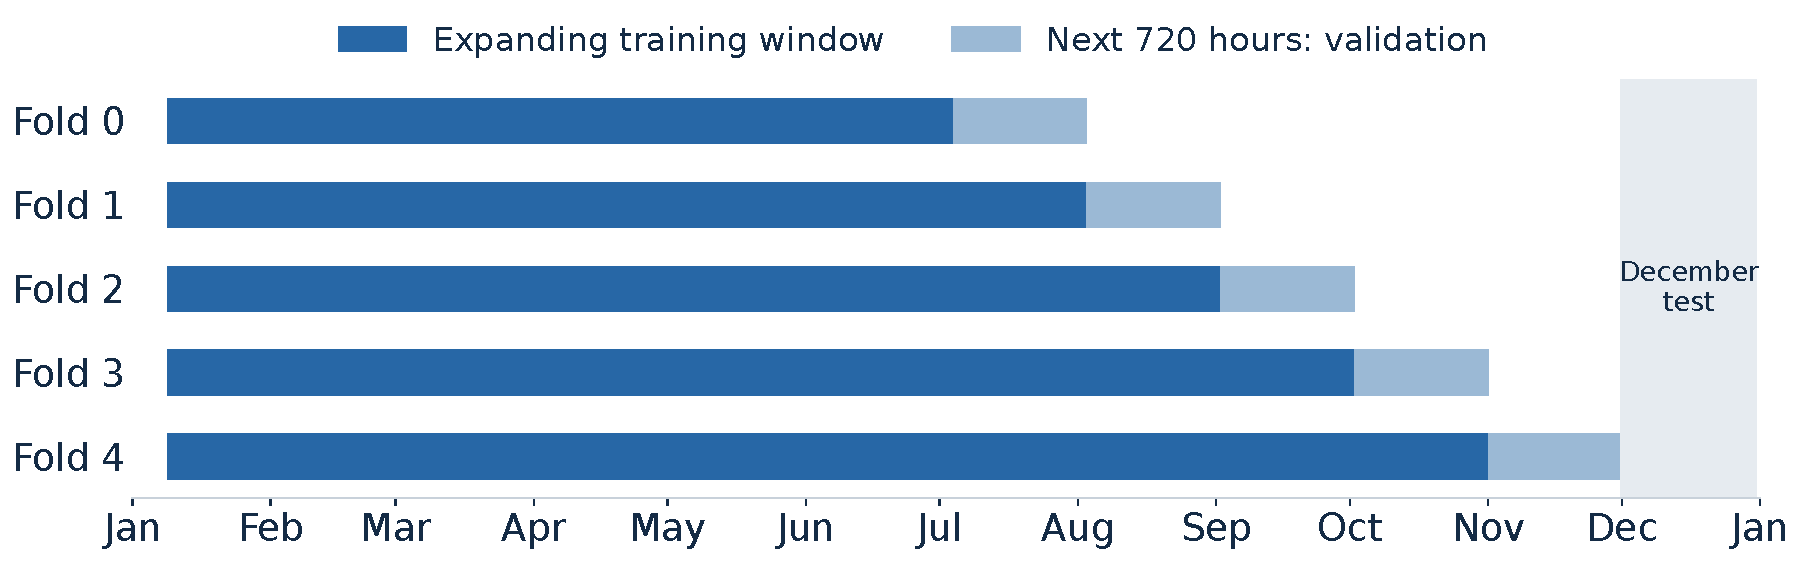
\includegraphics[width=\textwidth,height=3.55cm,keepaspectratio]{slides/figures/chronological_cv.pdf}\par
\raggedright
{\small After history warm-up, five expanding windows each validate the next 30 days.\par
Selection: lowest mean CV RMSE $\rightarrow$ refit on all development data $\rightarrow$ December.\par
\color{Muted}Tuning and reporting reuse folds (no nested CV); zero gap assumes prompt data.}
\end{frame}

% MAIN 10 -- 55 seconds
\begin{frame}{Learn the load level---or a correction to yesterday}
\vspace{2mm}
\begin{columns}[t,onlytextwidth]
\column{.47\textwidth}
\tagline{TWO SEASONAL BASELINES}
\[\widehat y_t=y_{t-24}\qquad\widehat y_t=y_{t-168}\]
\tagline{FIVE REGRESSION FAMILIES}
{\small Linear regression / tuned Ridge\par
Decision tree (DT)\par
Random forest (RF)\par
RBF support vector regression (SVR)\par
XGBoost (XGB)}
\column{.49\textwidth}
\tagline{TWO TARGET FORMULATIONS}
\textbf{Absolute:}\quad learn $y_t$.\par\vspace{3mm}
\textbf{Residual ($\Delta$):}
\[r_t=y_t-y_{t-24}\]
\[\widehat y_t=y_{t-24}+g(\mathbf{x}_t)\]
{\small Learn the change from yesterday so recent load carries the current level.}
\end{columns}
\takeaway{Both target formulations compete on development CV.}
{\small\color{Muted}RF averages are range-bounded; boosted trees do not share this strict bound.}
\end{frame}

% MAIN 11 -- 65 seconds
\begin{frame}{Why predict a correction? July tests extrapolation}
\setlength{\parskip}{2pt}
\tagline{FOLD 0: 4 JULY--2 AUGUST \quad / \quad TUNED MODELS}
\begin{columns}[t,onlytextwidth]
\column{.47\textwidth}
\textbf{A new load range}\par
{\small Training maximum: \textbf{110,711 kW}\par
Validation maximum: \textbf{133,130 kW}\par
About \textbf{12\%} of hours exceed the training maximum.\par
For $r_t=y_t-y_{t-24}$, \textbf{0\%} fall outside the training residual range.}
\column{.49\textwidth}
\textbf{July-fold RMSE (kW)}\par
\begin{tabular}{@{}lrr@{}}
\toprule Model & Absolute & Residual\\\midrule
RF & 5,554 & \textbf{3,215}\\
XGBoost & 5,344 & \textbf{2,979}\\\bottomrule
\end{tabular}\par\vspace{1mm}
{\small RF averages cannot extrapolate beyond training targets. Learning a correction reduces the impact of the level shift.}
\end{columns}
\takeaway{Residual learning is not necessary for the selected SVR.}
{\small SVR CV: absolute \textbf{2,411} vs residual \textbf{2,427 kW}; nearly tied.\par
Target variants were tuned separately; gains also reflect their chosen parameters.}
\end{frame}

% MAIN 12 -- 90 seconds
\begin{frame}{Absolute SVR leads CV, with close alternatives}
\setlength{\parskip}{2pt}
{\small Randomized search: \textbf{170 configurations $\times$ 5 temporal folds per target type};\par
SVR CV RMSE fell \textbf{39.3\%} versus default SVR. {\color{Muted}Bergstra \& Bengio (2012).}}
\begin{columns}[c,onlytextwidth]
\column{.63\textwidth}
\fig{slides/figures/cv_ranking.pdf}{3.85cm}
\column{.33\textwidth}
\metric{\CVRMSE}{kW mean CV RMSE}
{\small $\pm$ \CVSD{} kW fold SD.\par
\textbf{Default models:} XGB wins November; LR (\textbf{2,792 kW}) wins five-fold CV.\par
SVR and DT trail Naive-24h (\textbf{3,392 kW}) on CV.}
\end{columns}
{\small\textbf{More recent history: h24 vs h1 (CV).} SVR \CVRMSE{} $\rightarrow$ \HoneRMSE{} kW ($-22.6\%$).\par
\color{Muted}Same configurations/dates; histories and initial rows differ. CV folds are reused.}
\end{frame}

% MAIN 13 -- 65 seconds
\begin{frame}{Daily lags drive accuracy; the expanded set hurts}
\setlength{\parskip}{3pt}
\tagline{ABSOLUTE-TARGET RF / FIVE-FOLD CV / FIXED D-TUNED PARAMETERS}
{\small\renewcommand{\arraystretch}{1.08}
\begin{tabularx}{\textwidth}{@{}lXrrr@{}}
\toprule Set & Feature group & Inputs & RMSE (kW) & Change\\\midrule
A & Weather only & 5 & 15,010 & ---\\
B & + Calendar & 12 & 10,041 & $-33.1\%$\\
C & + Special days & 15 & 9,168 & $-8.7\%$\\
\textcolor{Blue}{\textbf{D}} & \textcolor{Blue}{\textbf{+ Daily lags (24 h, 48 h)}} & \textcolor{Blue}{\textbf{17}} & \textcolor{Blue}{\textbf{3,010}} & \textcolor{Blue}{$-67.2\%$}\\
E & + Weekly lag and rolling summaries & 21 & 3,700 & $+22.9\%$\\\bottomrule
\end{tabularx}}\par
{\small\textbf{D is selected.} Daily lags give the largest gain; adding weekly/rolling features worsens RF.\par
XGBoost also worsens: \textbf{3,010 $\rightarrow$ 4,921 kW} (D $\rightarrow$ E).\par
\color{Muted}Possible mechanism: rolling levels may hinder July extrapolation. D/E does not isolate the weekly lag. E/F weather removal changes RMSE by up to 5.3\%; this is not an SVR test.}
\end{frame}

% MAIN 14 -- 65 seconds
\begin{frame}{The selected SVR halves daily-baseline December RMSE}
\begin{columns}[c,onlytextwidth]
\column{.70\textwidth}
\fig{slides/figures/december_comparison.pdf}{4.45cm}
\column{.26\textwidth}
\metric{\GainDaily\%}{RMSE reduction vs Naive-24h}
\vspace{4mm}
{\small\textbf{\GainWeekly\%} vs Naive-168h\par
MAE: \textbf{\TestMAE{} kW}\par
MAPE: \textbf{\TestMAPE\%}\par
$R^2$: \textbf{\TestRtwo}}
\end{columns}
\takeaway{Residual SVR: observed test-best; not CV-selected. Absolute SVR remains final.}
{\small December 1--30 only; results condition on observed target-hour weather.}
\end{frame}

% MAIN 15 -- 55 seconds
\begin{frame}{Good daily tracking still leaves concentrated errors}
\centering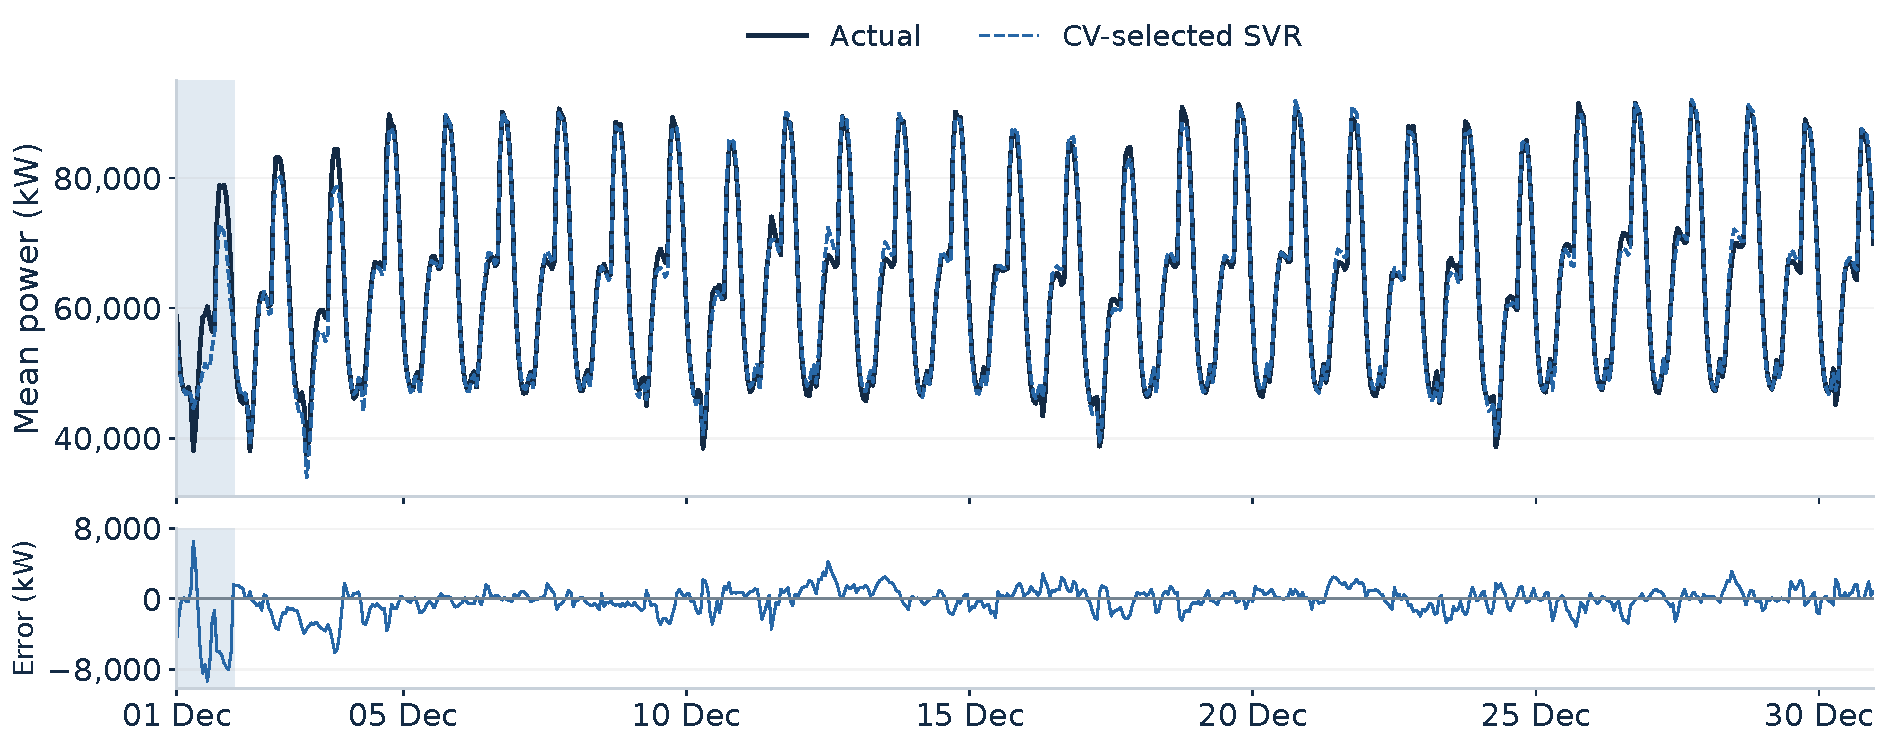
\includegraphics[width=\textwidth,height=4.65cm,keepaspectratio]{slides/figures/december_trace.pdf}\par
\raggedright
\begin{columns}[t,onlytextwidth]
\column{.35\textwidth}
{\small\textbf{Bias: \Bias{} kW}\par Error = forecast $-$ actual.}
\column{.61\textwidth}
{\small\textbf{Worst day: 1 December (Mawlid)}\par MAE \WorstMAE{} kW; highlighted in blue.}
\end{columns}
{\small\color{Muted}Possible explanation: the holiday flag may transfer larger Eid demand reductions to Mawlid.}
\end{frame}

% MAIN 16 -- 50 seconds
\begin{frame}{Evaluation shortcuts change what the score means}
\setlength{\parskip}{2pt}
\tagline{A CONCRETE LEAKAGE MECHANISM IN THE SHUFFLED DIAGNOSTIC}
{\centering
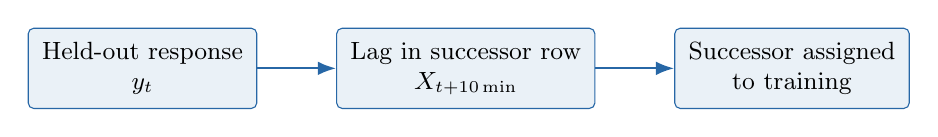
\begin{tikzpicture}[node distance=10mm,>=Latex,
 box/.style={draw=Blue,fill=Pale,rounded corners=2pt,align=center,inner sep=5pt,font=\small}]
\node[box] (a) {Held-out response\\$y_t$};
\node[box,right=of a] (b) {Lag in successor row\\$X_{t+10\,\mathrm{min}}$};
\node[box,right=of b] (c) {Successor assigned\\to training};
\draw[->,thick,Blue] (a)--(b);\draw[->,thick,Blue] (b)--(c);
\end{tikzpicture}
\par}
\vspace{1mm}
{\small\textbf{Separate RF tuning diagnostic} (20 candidates; errors in kW)}\par
{\renewcommand{\arraystretch}{1.10}\begin{tabularx}{\textwidth}{@{}Xrr@{}}
\toprule
CV strategy & CV estimate & December test\\\midrule
Shuffled KFold & 2,007.6 & 2,173.6\\
Expanding TimeSeriesSplit & 3,012.4 & 2,044.2\\\bottomrule
\end{tabularx}}\par\vspace{1mm}
{\small\color{Blue}\bfseries Same Random Forest: shuffled 10-min split $R^2$ 0.999 vs chronological h24 $R^2$ 0.980.}\par
{\small\color{Muted}Forecast settings, features and test sets differ; this is a descriptive comparison.}
\end{frame}

% MAIN 17 -- 45 seconds
\begin{frame}{Findings \& limitations}
\setlength{\parskip}{2pt}
\tagline{FINDINGS}
{\small
\begin{enumerate}
\setlength{\itemsep}{3mm}
\item Choose the final model on chronological CV; report December separately.
\item Daily lags give the largest RF gain; weekly/rolling features hurt.
\item The CV-selected SVR halves December Naive-24h error (\textbf{$-50.7\%$}).
\end{enumerate}}
\vspace{3mm}
\tagline{LIMITATIONS}
{\small
\begin{itemize}
\setlength{\itemsep}{2mm}
\item Weather is observed, not forecast; prompt recent-load measurements assumed.
\item One city, one year, one 30-day test.
\end{itemize}}
\takeaway{Next: issuance-time weather and independent seasonal tests.}
\end{frame}

% MAIN 18 -- 20 seconds
\begin{frame}{Conclusion \& Q\&A}
\vspace{6mm}
\tagline{CV-SELECTED ABSOLUTE-TARGET SVR \quad / \quad DECEMBER 2017}
\vspace{4mm}
\begin{columns}[c,onlytextwidth]
\column{.47\textwidth}
\metric{\TestRMSE{} kW}{RMSE on 720 hourly observations}
\column{.47\textwidth}
\metric{\GainDaily\%}{lower RMSE than Naive-24h}
\end{columns}
\vspace{8mm}
\textbf{A promising chronological benchmark, conditional on observed weather.}\par
\vspace{7mm}
{\color{Blue}\fontsize{17}{21}\selectfont\bfseries Thank you. Questions?}
\end{frame}

\end{document}
